%%%%%%%%%%%%%%%%%%%%%%%%%%%%%%%%%%%%%%%%%%%%%%%%%%%%%%%%%%%%%%%%%%%%%%%%%%%%%
%%%
%%% File: utthesis2.doc, version 2.0jab, February 2002
%%%
%%% Based on: utthesis.doc, version 2.0, January 1995
%%% =============================================
%%% Copyright (c) 1995 by Dinesh Das.  All rights reserved.
%%% This file is free and can be modified or distributed as long as
%%% you meet the following conditions:
%%%
%%% (1) This copyright notice is kept intact on all modified copies.
%%% (2) If you modify this file, you MUST NOT use the original file name.
%%%
%%% This file contains a template that can be used with the package
%%% utthesis.sty and LaTeX2e to produce a thesis that meets the requirements
%%% of the Graduate School of The University of Texas at Austin.
%%%
%%% All of the commands defined by utthesis.sty have default values (see
%%% the file utthesis.sty for these values).  Thus, theoretically, you
%%% don't need to define values for any of them; you can run this file
%%% through LaTeX2e and produce an acceptable thesis, without any text.
%%% However, you probably want to set at least some of the macros (like
%%% \thesisauthor).  In that case, replace "..." with appropriate values,
%%% and uncomment the line (by removing the leading %'s).
%%%
%%%%%%%%%%%%%%%%%%%%%%%%%%%%%%%%%%%%%%%%%%%%%%%%%%%%%%%%%%%%%%%%%%%%%%%%%%%%%

%%%%%%%%%%%%%%%%%%%%%%%%%%%%%%%%%%%%%%%%%%%%%%%%%%%%%%%%%%%%%%%%%%%%%%%%%%%%%
%%%
%%
%% This file, and the corresponding tcdthesis.sty the accompanied it, have
%% been modified for the M.Sc. styles used in Trinity College, Dublin
%%
%%
%%%%%%%%%%%%%%%%%%%%%%%%%%%%%%%%%%%%%%%%%%%%%%%%%%%%%%%%%%%%%%%%%%%%%%%%%%%%%
\documentclass[a4paper, 12pt, oneside]{report}         %% LaTeX2e document.
\usepackage {tcdthesis}              %% Preamble.

\mastersthesis                       %% Uncomment one of these; if you don't
% \phdthesis                         %% use either, the default is \phdthesis.

\thesisdraft                         %% Uncomment this if you want a draft
                                     %% version; this will print a timestamp
                                     %% on each page of your thesis.

\leftchapter                         %% Uncomment one of these if you want
% \centerchapter                     %% left-justified, centered or
% \rightchapter                      %% right-justified chapter headings.
                                     %% Chapter headings includes the
                                     %% Contents, Acknowledgments, Lists
                                     %% of Tables and Figures and the Vita.
                                     %% The default is \centerchapter.

% \singlespace                       %% Uncomment one of these if you want
\oneandhalfspace                     %% single-spacing, space-and-a-half
% \doublespace                       %% or double-spacing; the default is
                                     %% \oneandhalfspace, which is the
                                     %% minimum spacing accepted by the
                                     %% Graduate School.

\renewcommand{\thesisauthor}{Jane Doe}                %% Your official TCD name.
\renewcommand{\thesismonth}{August}                   %% Your month of graduation.
\renewcommand{\thesisyear}{2021}                      %% Your year of graduation.
\renewcommand{\thesistitle}{Your Title here}          %% The title of your thesis; use mixed-case.
\renewcommand{\thesisauthorpreviousdegrees}{, BAI}    %% Your previous degrees, abbreviated; separate multiple degrees by commas.
\renewcommand{\thesissupervisor}{Sean Doe}            %% Your thesis supervisor; use mixed-case and don't use any titles or degrees.
% \renewcommand{\thesiscosupervisor}{}                %% Your PhD. thesis co-supervisor; if any.

% \renewcommand{\thesiscommitteemembera}{}
% \renewcommand{\thesiscommitteememberb}{}
% \renewcommand{\thesiscommitteememberc}{}
% \renewcommand{\thesiscommitteememberd}{}
% \renewcommand{\thesiscommitteemembere}{}
% \renewcommand{\thesiscommitteememberf}{}
% \renewcommand{\thesiscommitteememberg}{}
% \renewcommand{\thesiscommitteememberh}{}
% \renewcommand{\thesiscommitteememberi}{}


\renewcommand{\thesisauthoraddress}{...}

\renewcommand{\thesisdedication}{...}     %% Your dedication, if you have one; use "\\" for linebreaks.


%%%%%%%%%%%%%%%%%%%%%%%%%%%%%%%%%%%%%%%%%%%%%%%%%%%%%%%%%%%%%%%%%%%%%%%%%%%%%
%%%
%%% The following commands are all optional, but useful if your requirements
%%% are different from the default values in tcdthesis.sty.  To use them,
%%% simply uncomment (remove the leading %) the line(s).

\renewcommand{\thesisdegree}{Master of Science in Computer Science}
                                     %% default is "DOCTOR OF PHILOSOPHY"
                                     %% for \phdthesis or "MASTER OF ARTS"
                                     %% for \mastersthesis.  Provide the
                                     %% correct FULL OFFICIAL name of
                                     %% the degree.
\renewcommand{\thesisdegreestream}{ (Data Science)}
                                     %% Default is empty. This is used on
                                     %% the title page of the thesis.

\renewcommand{\thesisdegreeabbreviation}{M.Sc.}
                                     %% Use this if you also use the above
                                     %% command; provide the OFFICIAL
                                     %% abbreviation of your thesis degree.
\renewcommand{\thesistype}{Dissertation}    %% Use this ONLY if your thesis type
                                     %% is NOT "Thesis" for \phdthesis
                                     %% or \mastersthesis.
                                     %% Provide the OFFICIAL type of the
                                     %% thesis; use mixed-case.

%%%
%%%%%%%%%%%%%%%%%%%%%%%%%%%%%%%%%%%%%%%%%%%%%%%%%%%%%%%%%%%%%%%%%%%%%%%%%%%%%

\usepackage{graphicx,color}
\usepackage{anysize}
\usepackage{amsmath}
\usepackage{natbib}
\usepackage{caption}
\usepackage{hyperref}
\usepackage{listings}
\usepackage{float}

%%------------------------------------------------
%% Listing macros
%%------------------------------------------------
%% Examples for the commands in the document below
%%
%% includecode:
%% \includecode{caption for table of listings}{caption for reader}{filename}
%% - includes a file with code and adds a caption that should describe the code in some detail and a shorter caption for the table of listings
\newcommand{\includecode}[4]{\lstinputlisting[floatplacement=H, caption={[#1]#2}, captionpos=b, frame=single, label={#3}]{#4}}

%%------------------------------------------------
%% Image macros
%%------------------------------------------------

%% includescalefigure:
%% \includescalefigure{label}{short caption}{long caption}{scale}{filename}
%% - includes a figure with a given label, a short caption for the table of contents and a longer caption that describes the figure in some detail and a scale factor 'scale'
\newcommand{\includescalefigure}[5]{
\begin{figure}[htb]
\centering
\includegraphics[width=#4\linewidth]{#5}
\captionsetup{width=.8\linewidth} 
\caption[#2]{#3}
\label{#1}
\end{figure}
}

%% includefigure:
%% \includefigure{label}{short caption}{long caption}{filename}
%% - includes a figure with a given label, a short caption for the table of contents and a longer caption that describes the figure in some detail
\newcommand{\includefigure}[4]{
\begin{figure}[htb]
\centering
\includegraphics{#4}
\captionsetup{width=.8\linewidth} 
\caption[#2]{#3}
\label{#1}
\end{figure}
}





\begin{document}                                  %% BEGIN THE DOCUMENT

\thesistitlepage                                  %% Generate the title page.

%\hypersetup{pageanchor=false}
%\thesisdeclarationpage                            %% Generate the declaration page.

%\thesispermissionpage                             %% Generate the copyright permission page
%\hypersetup{pageanchor=true}

\begin{thesisabstract}                            %% the abstract for your thesis
...ABSTRACT...
\end{thesisabstract}

%\thesisdedicationpage                            %% Generate the dedication page.

\begin{thesisacknowledgments}                     %% Use this to write your
  Thank you Mum \& Dad.                           %% acknowledgments; it can be anything
\end{thesisacknowledgments}                       %% allowed in LaTeX2e par-mode.
  
  
\tableofcontents                                  %% Generate table of contents.
\listoftables                                     %% Uncomment this to generate list of tables.
\listoffigures                                    %% Uncomment this to generate list of figures.

%%
%% Include thesis chapters here...
%%
\chapter{Introduction}

Here are summaries of the papers I have read thus far

\section{Background for GAEN keys}
\label{sec:BackgroundGAENKeys}

Background

The first paper is Contact Tracing App Privacy: What Data Is Shared
By Europe’s GAEN Contact Tracing Apps~(\cite{9488728}). This paper discusses the data sent to back end servers of various contact tracing apps in Europe. The apps have two components: the 'client' app which is controlled by the national public health authority and the GAEN service that, on android, is managed by Google as part of the Google Play services. The paper investigates both of these components. It found that the Google Play services component continuously sends requests to the Google servers which contain information such as the phone IMEI, handset hardware serial number, SIM serial number, etc. This may be considered intrusive , however most users would have accepted this data sharing if that had previously enabled Google Play services. This data sharing is not specific to the covid tracing app. There may be a way to identify a user is  specific data is sent in every request. There are experiments run to test the data being sent by different apps. 

The paper CoAvoid: Secure, Privacy-Preserved Tracing of
Contacts for Infectious Diseases~(\cite{9908579}) discusses the privacy and security concerns of covid tracing apps and proposes its own CoAvoid app which improves on these issues. It talks about how inappropriate uses of the GAEN API may expose all information about confirmed patients to servers and relevant users. This may allow someone to gather lots of information about patients and discover their identities, daily routines or social relationships. Due to a limitation of BLE, it may be possible for attackers to send users excess false alarms and put further strain on the public health system (wormhole attack). It talk about how the BLE to calculate if two devices came into contact can be affected by factors such as environment, transmitting power, receiving sensitivity, etc. The GAEN design is vulnerable to profiling, possibly de-anonymising infected persons and wormhole attacks. It describes how the GAEN app works: It randomly generates a Daily Tracking Key (DTK), a unique identifier used for 24 hours. It uses function {\it f} to derive the Rolling Proximity Identifier (RPI) based on the DTK. These identifiers are sent in Bluetooth Advertisements, which will be replaced every 20 minutes. The apps simultaneously collects and stores other users RPIs locally. If a user test positive, their DTK is uploaded to a central server. Other download these DTKs and reconstruct the RPIs. They compare these to their local list of keys. The authenticity of the information being downloaded cannot be verified and thus wormhole attacks may occur. The paper further describes two types of potential attacks: Wormhole and Privacy Analysis attack. It may be possible to identify things about a user by tracking the DTK uploads.

The paper Digital Contact Tracing Solutions: Promises, Pitfalls
and Challenges~(\cite{9931613}) analyses digital contact tracing solutions. It discusses the security and privacy issues with GAEN. It proposes its own solution called TraceCorona. Apple and Google collaborated to create a decentralised contact tracing interface calle Exposure Notification API (GAEN). Access to the API has been given to only one organisation authorised by the government. BLE is used for sensing the proximity between individual devices. The phones send out information like temporary identifiers (TempIDs) that can be sensed by other devices. It also records signal strength in an attempt to estimate the distance of the encounter. It discusses requirements of accuracy, superspreader and accountability for a digital contact tracing system to be acceptable.

The article Privacy and Integrity Threats in Contact
Tracing Systems and Their Mitigations~(\cite{9928557}) reports privacay and integrity threats in GAEN and proposes a new system called Pronto-B2. Threats to security and privacy include the possibility of tracing and deanonymising citizens using passive devices and injecting false at-risk alerts. An attacker may trace a user by linking locations visited by the same user. They may also try to deanonymise users by linking locations visited by users to their real identities. 'Paparazzi Attack': using passive devices, the attacker can catch and store the pseudonyms of a target user. They can link together the passive devices recieved the pseudonyms belonging to the same user. The attacker can obtain information about the habits of an infected user and use it for economical gain. 'Brutus Attack': The attacker colludes with the server and the health authority to discover which user uploaded certain data. Pseudonyms in GAEN are called rolling proximity identifiers (RPIs). A short random secret called Temporary Exposure key (TEK) is generated each day by the smartphone. All RPIs of a given day of a user are generated by running a PRF on the input TEK.

The paper October 2020 Survey of GAEN App Key Uploads~(\cite{survey}) is a survey of the TEKs published across 8 European regions. It estimates the number of users uploading TEKs and compares this to the expected number based on population, number of active users and covid case counts. It reports a shortfall of uploads in a number of regions. The efficacy of these apps remains unclear.

\section{Background for how GAEN keys are Generated}
\label{sec:BackgroundGAENKeysGeneration}
\begin{figure}
    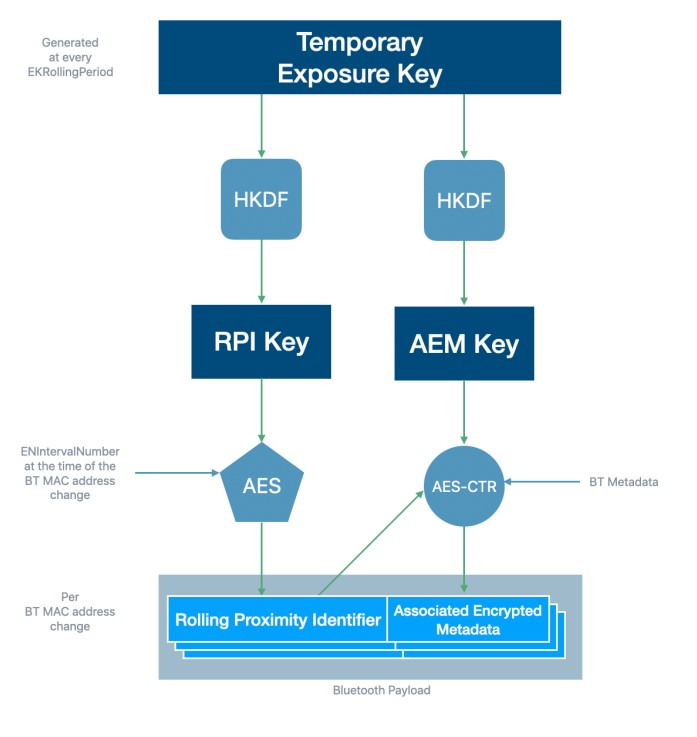
\includegraphics[width=\linewidth]{generatedKEY.jpg}
    \caption{How the GAEN key is generated}
    \label{fig:keyGeneration}
\end{figure}

Here is how the keys are generated. 

The documentation from Google and Apple~(\cite{appleCrypto}) found online details how the GAEN keys are encrypted. An ENIntervalNumber is calculated every 10 minutes, it is a 32-bit unsigned little endian value. The TEKRollingPeriod is how long the Temporary Exposure Key is valid, it is 24 hours. The Temporary Exposure Key is generated and associated with an ENIntervalNumber. It is generated as a 16-byte value using CRNG, which is a cryptographic number generator. At the end of every TEKRollingPeriod, a new key is generated. The Rolling Proximity Identifier Key (RPIK) is derived from the TEK. It is derived by RPIKi ← HKDF(teki, NUL L, UTF8("EN-RPIK"),16), where the HKDF function is as detailed in ~(\cite{rfc5869}), which uses the SHA-256 hash functions. The Rolling Proximity Identifiers are privacy preserving identifiers that are broadcast in Bluetooth payloads. Each time the MAC address changes a new Rolling Proximity Identifier is generated using the Rolling Proximity Identifier Key using RPIi, j ← AES128(RPIKi, PaddedDataj). The use of 16-byte identifiers result in a low probability of collisions and limits the risk of false positive matches. The associated encrypted metadata is encrypted with the Rolling Proximity Identifier. 


\section{Background for Tests for Randomness}
\label{sec:BackgroundTests}

The paper Randomness testing of modern encryption techniques in cloud environment~(\cite{6236554}) compares different modern encryption techniques on a traditional desktop and in a cloud environment. It tests 8 algorithms, including AES which is used in GAEN. It uses the NIST statistical test package which contains 15 tests, listed in the paper. It implements the tests in Java. It runs the NIST tests which produces P-values, which are rejected if they are less than 0.01. There is a max rejection rate, 4 in this paper, there is an equation to calculate this. It runs these tests on all the algorithms and outputs its results. It doesn't find any problems with the algorithms but there are differences when they are ran on the desktop environment versus in the cloud. 

The paper Effectiveness Analysis of Encrypted and Unencrypted Bit Sequence Identification Based on Randomness Test~(\cite{7406118}) uses statistical tests to identify whether a bit sequence is encrypted or unencrypted. Randomness tests are used to evaluate the security of cipher algorithms. It uses the SP800-22 rev1a standard. The standard contains 15 randomness tests but this paper uses 5 of them, frequency test, frequency test within a block, runs test, longest runs of one in a block and cumulative sums test. It provides analysis on some of these tests, frequency, runs, frequency within a block. It describes the P-value used and how it is calculated. It somewhat accurately classifies a bit sequence as encrypted or unencrypted.

The paper Analyzing of Chaos based Encryption with Lorenz and Henon Map~(\cite{8653652})

The paper Statistical Analysis of Enhanced SDEx Encryption Method Based on SHA-512 Hash Function~(\cite{9209663}) performs statistical analysis on an enchanced SDEx method based on the SHA-512 hash function. It uses NIST and carries out four tests: frequency, block frequency, cumulative sum and runs. The algorithm passes all the test, it gets a P-value of > 0.01. It could not do the compression tests from NIST as the size of the test files was too small so it uses WINRAR. It says that of the file is a string of random bits then it should be able to be compressed. It checks that the size of the file before and after compression using WINRAR is the same. The algorithm passes this test also. References a paper about the cryptanalysis of the SDEx method, should read as this paper only does the statistical analysis.

The paper Analysis of the Randomness Performance of the Proposed Stream Cipher Based Cryptographic Algorithm~(\cite{9232553}) does randomness testing on an adapted version of the Vernam Cipher. It uses NIST to do cumulative sums, runs, longest run of ones and frequency tests. It mentions other test suits called NIST STS, Dieharder and TestU01. Mentions Strict Avalanche Criterion (SAC) testing but i do not think this is relevant to the GAEN keys. The cumulative sum is a test concentrates on determining the maximal excursion from zero of the random walk described by the increasing amount of adjusted (-1, +1) digits in the sequence. The Runs Test was utilized to verify whether the total numbers of runs of ones and zeros of various lengths areas projected for a random sequence. The longest run was to define whether the longest run of ones within an M-bit block of the tested sequence is consistent with the length of the longest run of ones anticipated in a random sequence of M bits. For a pseudorandom number generator, the number of ones and zeros in the output must be equal. A test that determines the proportions of zeros and ones for the entire sequence is the Frequency test.

The paper On the Robustness of RSA-OAEP Encryption and RSA-PSS Signatures Against (Malicious) Randomness Failures~(\cite{10.1145/3052973.3053040}) analyses the robustness of the RSA-OAEP encryption scheme and the RSA-PSS signature scheme. The paper gives examples of real world randomness failures but it focused on the enc scheme and signature thing rather than the randmoness of the key itself. It's a very technical paper that I do not fully understand and do not think its discussion of randmoness tests is relevant to the GAEN kesy testing. It is very theoretical. Mentions random oracle model and repeated randmoness and collision resistant? 

The paper Evolving boolean functions for fast and efficient randomness testing~(\cite{10.1145/3205455.3205518}) is VERY USEFUL paper. Introduces a new boolean function for testing randomness, s a novel method for the statistical randomness testing of cryptographic primitives, which is based on the evolutionary construction of the so-called randomness distinguisher. Each distinguisher is represented as a Boolean polynomial in the Algebraic Normal Form. It talks about evolutionary algorithms and their new Boolean functions operating as simple, but high-quality distinguishers of statistical (non)randomness in the data generated by cryptographic algorithms. These boolean functions can provide the same results as the usual test suites NIST etc, but faster and using less data.  The quality of each distinguisher was measured in terms of the so-called Z-score. Mentions another paper using a software package named Ent. In total, they evaluated seven statistics (entropy, compression, hisquared, arithmetic mean, pierror, excess and correlation) associated to five tests, resulting in an observation that studied statistics are not completely independent and could be reduced to five statistics. The paper goes on to describe their function but it is quite confusing and shows their results. Would definitely be worth looking at to test the GAEN keys.

The paper Recommendations on Statistical Randomness Test Batteries for Cryptographic Purposes~(\cite{10.1145/3447773}) is a VERY USEFUL paper. It compares the different batteries(test) suits like NIST, Dieharder, TestU01 and more. It lists the tests used in each one and explains them. It contains very useful references. Need to exam the keys and their structure and refer to this paper to begin deciding on a test suite and what test to run. Contains useful tables of pros and cons of each and compares the tests they have.

To ensure the strength and resilience of your encryption solutions ~(\cite{linkedInArticle}) against various attacks and threats, you need to measure and compare them using methods and tools such as simulations, audits, reviews, and assessments. For example, you might want to conduct security tests on key management to prevent key leakage, loss, or compromise; encryption mode to avoid weaknesses such as padding oracle attacks; cryptanalysis to detect or prevent brute force or side-channel attacks; and compliance with laws, regulations, standards, and best practices. By doing so, you can evaluate the performance and security of your encryption solutions and enhance their quality and effectiveness.

Article by OWASP~(\cite{OWASP}) might be useful.

Article by OWASP~(\cite{OWASP2}) about Insecure Randomness. Insecure randomness errors occur when a function that can produce predictable values is used as a source of randomness in security-sensitive context. Computers are deterministic machines, and as such are unable to produce true randomness. Pseudo-Random Number Generators (PRNGs) approximate randomness algorithmically, starting with a seed from which subsequent values are calculated.

Wikipedia page~(\cite{WIKI}) on Randomness test. Mentions famous PRNG that fails randomness test https://en.wikipedia.org/wiki/RANDU . Though there are commonly used statistical testing techniques such as NIST standards, Yongge Wang showed that NIST standards are not sufficient. Furthermore, Yongge Wang(http://webpages.uncc.edu/yonwang/) designed statistical-distance-based and law-of-the-iterated-logarithm-based testing techniques. Using this technique, Yongge Wang and Tony Nicol("Statistical Properties of Pseudo Random Sequences and Experiments with PHP and Debian OpenSSL") detected the weakness in commonly used pseudorandom generators such as the well known Debian version of OpenSSL pseudorandom generator which was fixed in 2008.  The use of Hadamard transform (https://en.wikipedia.org/wiki/Hadamard-transform) to measure randomness was proposed by S. Kak and developed further by Phillips, Yuen, Hopkins, Beth and Dai, Mund, and Marsaglia and Zaman, On the Complexity of Pseudo-Random Sequences or If You Can Describe a Sequence It Can't be Random. Advances in Cryptology. 

\section{Approaches for Testing for Randomness}
\label{sec:TestApproachs}

Below is a list of potential test approachs for my dissertation, and tests I should consider
\begin{itemize}
    \item NIST, Dieharder, TestU01~(\cite{10.1145/3447773}) INCLUDE at least 1
    \item chi-squared test, Entropy measurement INLCUDED above
    \item Boolean functions~(\cite{10.1145/3205455.3205518}) INCLUDE
    \item Hilbert curve and heatmap, mentioned in tek transparency reports. Analyse distrubutions, INCLUDE
    \item OpenSSL, Crypto++, PyCrypto, and JCE potentially~(\cite{linkedInArticle}) POSSIBLY include if relevent
    \item bias testing: Keys generated at specific times POSSIBLY include if I have time
    \item \sout{Hadamard spectral test}~(\cite{WIKI}) Used for linear congruential generators, not applicable
\end{itemize}
\chapter{State of the Art}

Give introduction

\section{Background}
Introduction

\subsection{What are GAEN Keys}
Introduction
\subsubsection{Contact Tracing Apps}
Google and Apple developed the Google/Apple Exposure Notification (GAEN) system to facilitate contact tracing in response to the Covid-19 Pandemic. (Mention conventional contact tracing). Nations across the world used this technology to create contract tracing apps, for example Covid Tracker in Ireland and SwissCovid in Switzerland~(\cite{9488728}).  \newline

The way the contact tracing works, if a user enables it, is as follows:
\begin{itemize}
    \item Every 10-20 minutes the user's device will generate a random 128-bit key, referred to as a Temporary Exposure Key (TEK). 
    \item The user's device will broadcast these keys using Bluetooth Low Energy (BLE). 
    \item The user's device will listen and store the TEKs being broadcasted from other devices within a certain radius. These TEKs are stored locally on the device.
    \item If a user tests positive for Covid, they can log this into the app. The app will send the user's recent TEKs (around the 14 days) to a central server managed by the local health authority.
    \item Every approx. 2 hours, the user's device will download the TEKs from the central server.
    \item The app compares these downloaded TEKs to the TEKs stored locally on the device.
    \item If there is a match, this means that the user has potentially been exposed to Covid and the app will notify them. 
    \item CITES
\end{itemize}

\subsubsection{Studies on GAEN-based Apps}

There have been numerous studies done on contact tracing apps that use GAEN technology. Google and Apple acknowledge that keeping users' information private and secure is essential to the success of the contact tracing app and claim to have designed their system with this central to the design ~(\cite{12345}).  Why is privacy so important for this app? Don't want to share covid status etc. \newline

The major privacy concerns of GAEN apps according to ~(\cite{9931613}) are the identification of users, tracking users or extracting the social graph of users. Contact tracing should aim to identify encounters rather than actual users, by doing so they should not leak any information that could be used to identify the user. Similarly, the data collected should not be able to be used to create the social graph of the user, the social connections and relationships of a user. Having this information could potentially result in the user being identified. \newline

Security is also a requirement for a contact tracing app according to ~(\cite{9931613}). The system should be resilient to large scale data pollution attacks. These could be fake exposure claims, where users may falsely claim they have been exposed in order to get out of work or another obligation or in an attempt to damage the reputation and credibility of the contact tracing apps. Fake exposure injection, a relay attack, may send users false notifications of potential exposures. The attacker could do this by capturing the TEKs of some user and broadcasting them in another location, leading to people being falsely notified of exposure. This could result in panic among users and the population, putting further strain on the healthcare system by creating a demand for unnecessary tests. It could also damage the trust in the contact tracing apps as their accuracy would be no longer trusted. \newline

~(\cite{9931613})  assess the GAEN apps on a variety of requirements. In terms of effectiveness, GAEN has been found to be imprecise at determining the distances between user devices (do i need to reference an internal reference?). Its use of BLE means scanning of the user's surroundings for other devices can only happen with frequent pauses to save battery life of the device. Many factors like positioning of the device's antenna, obstacles in the way and orientation of the device affect the computation of the distance between devices and the errors are significant. GAEN fails to account for 'superspreaders' of the virus, an individual who is very contagious and infects a number of other people. GAEN also does not have any mechanism for dealing with asymptomatic individuals, people that are infected with the virus and are contagious but do not show symptoms. Unknowingly, these people spread the virus. These individuals are unlikely to get tested and therefore won't log their infection in the app, meaning those that come in contact with them will not be notified of a potential exposure. This significantly impacts the effectiveness of the contact tracing apps. \newline

An investigation into the data shared by Europe's contact tracing apps that use GAEN ~(\cite{9488728}) discovered that a significant amount of data was being sent to Google servers. The android implementations of the GAEN systems use Google Play Services to facilitate GAEN-based contact tracing. The user must enable Google Play Services. It was found that Google Play Services connects to Google servers approximately every 20 minutes, sending requests that include the handset IP address, location data and persistent identifiers to link requests coming from the same device. The data sent to Google in other types of requests also include phone IMEI, device hardware serial number, SIM serial number and IMSI, phone number, WiFi MAC address, user email and Android ID. While sharing data to backend servers is not in itself an intrusion of privacy, the ability to link this data to a real-world user is problematic. Given that the user's IP address is being sent to Google very frequently, this could be used as location tracking. It is possible to de-anonymise this location data and potentially identify the user. Given that the user must enable Google Play Services, and therefore this data sharing, to do contact tracing, this does raise a concern to the privacy of the user. \newline

~(\cite{9928557}) examines several potential threats and privacy concerns of GAEN apps. They introduce a ‘paparazzi attack’ which involves using passive Bluetooth devices to capture the keys being broadcasted from a targeted user. If this user tests positive, the attacker can match their locally stored keys to those made publically available on the central server and learn that the user is positive for covid. This is a form of deanonymization. Similarly, an attacker could exploit the movements of a targeted user to gain money by linking the locations of the passive devices to the keys and sell this data to interested parties. \newline

The effectiveness of these GAEN contact tracing apps is undetermined ~(\cite{9488728})~(\cite{9931613}) 

Numerous alternative to the GAEN system have been proposed such as TraceCorona by ~(\cite{9931613}) in an attempt to remedy the above privacy and security concerns.


\subsection{What is Randomness}

In order to test for randomness/non-randomness we must first define what randomness is. A random bit sequence could be explained as the result of flipping an unbiased coin, with two sides 1 and 0, which has an equal chance of 50 percent of landing on side 1 or side 0. Each flip of the coin does not affect any future coin flips which means the flips are independent of each other. This unbiased coin can therefore be considered a perfect random bit stream generator as the appearances of 1s and 0s will be randomly and uniformly distributed. All elements in the sequence are independent of each other and future elements in the sequence cannot be predicted using previous elements ~(\cite{Nistdoc2}). This simple example gives us an understanding of what it means for a set of keys to be random. \newline

The keys must exhibit certain properties in order to be accepted as random. They should be independent meaning no previously generated keys affect a new key.  Equally likely meaning that  the probability of a 0 or 1 appearing at any point in the key is equal to 1/2. Scalable meaning that if the key is random, then any extracted subsequence is also random. ~(\cite{10.1145/3390525.3390540})Any indication of a dependency or bias within the data would indicate nonrandomness. \newline

\section{Literature Review}

Introduction

\subsection{How to Test for Randomness}

It is important to note that you can not say for certain whether something is random or not, you can only find evidence against non-randomness. It is not possible to give theoretical proof of randomness of a sequence. ~(\cite{55555}) Various statistical tests can be performed on the data in an attempt to compare and evaluate the data against a truly random sequence since the outcome when a statistical test is applied to a truly random sequence is known. ~(\cite{1195701}). \newline

A challenge when testing for randomness is that there is no agreed upon complete set of statistical tests to deem a sequence random ~(\cite{1195701}). There is an infinite number of tests that you could run in order to find the presence or absence of a pattern or bias within the data. The existence of a pattern or bias within the data would indicate that it is non randomness. \newline


\subsubsection{Hypothesis Testing}

Statistical testing is used to test against a defined null hypothesis (h0). The null hypothesis in this case is that the keys being tested are random. The alternative hypothesis (h1) is that the keys are not random. The challenge here is to determine which of these hypotheses can be accepted ~(\cite{10.1145/3447773}) . For each statistical test run on the data, the result accepts or rejects the null hypothesis. \newline

The following table shows the possible results on a hypothesis test:
 <table> ~(\cite{1195701}) \newline

The above situations are somewhat unknown but some control can be gained by knowing the probability of each of the error situations. The probability of Error Type 1 is defined as a, the level of significance ~(\cite{10.1145/3447773}). This value is typically 0.01, 0.05 or 0.10. The probability of Error Type 2 is defined as B, referred to as contrast power and is usually used as 1-B. ~(\cite{10.1145/3447773}). If the data is truly random, rejecting the null hypothesis, determining that the data is non-random, will occur a small percentage of the time. For example if a is 0.01, it would be expected that 1 sequence in 100 sequences is rejected ~(\cite{1195701}). \newline

In practice, p-values are used to reject or accept the null hypothesis. In the context of this project, a p-value can be defined as the probability that a key produced is less random than the keys previously tested, given the kind of non-randomness the test is assessing ~(\cite{1195701}). NEED TO FIX. A p-value equal to 1 indicates that the data is perfectly random while a p-value equal to 0 indicates that the data is completely non random. If the p-value is greater than or equal to a, the null hypothesis is accepted and the data appears to be random. If the p-value is less than a, the null hypothesis is rejected and the data is deemed non random. \newline

Maybe K-S stuff here or later on
TALK ABOUT test suites and what they are, not specific to one

\subsection{Studies on Randomness Testing}
Intro something like many examples of randomness testing being used on cryptographic techniques/applications. Multiple applications \newline

Given that encryption is essential for maintaining data security in cloud computing, ~(\cite{6236554}) performed randomness testing on eight modern encryption techniques, including AES, MARS and DES. They tested on two different platforms, desktop computer and Amazon EC2 Micro Instance. They evaluated the encryption techniques implemented as Pseudo Random Number Generators (PRNGs). They used the NIST Test Suite to perform the randomness testing. With a significance level of 0.01, any p-value less than 0.01 meant that sequence was rejected. They found no strong evidence of any statistical non randomness across the 8 encryption algorithms however some differences were found between them on the two different platforms. \newline

Statistical analysis has been run on an enhanced SDEx encryption method based on the SHA-512 hash function ~(\cite{9209663}). Using various tests like frequency, cumulative sums and runs, with a significance level of 0.01, it was found that this encryption algorithm was sufficiently random and passed the tests. They concluded that this SDEx method based on the SHA-512 hash function was quicker and equally or more secure than AES with a 256-bit key. They hope to use this method to secure end-to-end encryption for data transfer.\newline

Similarly, statistical tests for randomness have been run on new algorithms, like a proposed stream cipher cryptographic algorithm based on the popular Vernam Cipher ~(\cite{9232553}). The algorithm had a success rate of 99.5 percent across the statistical tests performed on it, which included frequency and longest runs of one's tests. Due to this success, the paper deemed the proposed algorithm effective in producing a random ciphertext sequence and detailed further work of implementing it to help secure medical records. \newline

SHA256 is vulnerable to length extension attacks which involve misusing particular hashes as authentication codes and using them to include extra information. ~(\cite{33333}) introduces a new and improved padding scheme and hashing process for SHA256 to deal with this issue. To verify that the solution is cryptographically secure, statistical tests for randomness are performed on the output of the Message Digest. Tests such as monobit frequency, frequency within a block and runs were carried out on the data. The results validate that the number of ones and zeros are randomly distributed in the final hash value. \newline

Statistical tests were also used to identify encrypted and unencrypted bit sequences ~(\cite{7406118}). Unencrypted bit sequences are less random than encrypted ones. From the SP800-22 rev1a standard, five tests were selected and a significance level of 0.01 was chosen.  If the sequence passes more than 3 of the tests, it was concluded that that sequence was encrypted. Otherwise the sequence was concluded as unencrypted. The results of the experiment were that 89 percent of the time, unencrypted sequences were identified correctly and 99 percent of the time encrypted sequences were identified correctly. \newline

\subsection{Examples of Randomness Failures}

Randomness failures pose a serious threat to cryptographic security ~(\cite{10.1145/3052973.3053040}). The consequences can be severe and there are many examples of real-world incidents. \newline

There are many examples of pseudo random number generators (PRNGs) failing and being guessable. Notably, the Debian Linux vulnerability in 2008 that left cryptographic keys to be guessable. It was caused by the code used to gather entropy, used to seed the PRNG used to create private keys, were removed. This resulted in only 32,768 possible keys meaning the connections made with these keys were insecure. CITE 11111 \newline

In 2015, Juniper Networks announced that there were multiple security vulnerabilities due to unauthorised code in their operating system, for their NetScreen VPN routers, called ScreenOS. CITE 22222 These vulnerabilities were due to Juniper's use of Dual EC (Elliptical Curve) as a PRNG. Dual EC had a weakness that was exploited in the Juniper incident. It was possible for an attacker, who knew the discrete logarithm of an input parameter Q with respect to a generator point, to see a number of consecutive bytes from the output and hence calculate the internal state of the generator. This allowed the attacker to predict all the future output of the generator. They were able to exploit this lack of randomness and passively decrypt VPN traffic.\newline

Bitcoin thefts in 2013 were due to a compromised PRNG used in Android wallets CITE 9999. Applications on Android using Java Cryptography Architecture (JCA) for key generation, signing and generating random numbers were not receiving cryptographically strong values because of an improper initialization of the underlying PRNG SecureRandom on Android devices CITE 991. The predictability of the values being generated by SecureRandom was exploited and attackers were able to guess the private keys used in Bitcoin Wallets and steal the Bitcoins the wallet contained. Again, attackers were able to exploit the lack of randomness.\newline

\section{Summary}
\chapter{Design}

\section{Challenges}
\subsection{Review of Test Suites}
There are a variety of statistical test suites that have been developed to test for randomness. In this section I will review these test suites in order to choose the appropriate one for this project's purposes. The notable test suites are Dieharder and NIST STS, being the most widely used and therefore most tested. \newline

Dieharder is a random number test suite which was designed to test RNGs used in a variety of applications such as cryptography and computer simulation. CITE rbgwebsite. It consists of 26 tests, extending the original Diehard battery which was created by George Marsaglia in 1995 ~(\cite{10.1145/3447773}). This testing suite is widely used ~(\cite{10.1145/3527157}) ~(\cite{10.1145/3398726}) ~(\cite{10.1145/3624991}) and is well tested. It is designed to be able to change the parameters in order to make failure unambiguous. It incorporates many of the tests in NIST STS. Because Dieharder is open source and encourages users to give feedback, contributions are continuously being made to improve and bug fix the tests. This results in a more reliable and stronger test suite than one that is closed or lacks a good feedback system like NIST STS CITE rgbwebsite. \newline 

NIST STS stands for the National Institute of Standards and Technology (NIST) Statistical Test Suite. It is used to test RNGs  used in applications such as cryptography, modelling and simulation CITE NISTdoc. It contains 15 tests and is widely used ~(\cite{6236554}) ~(\cite{9209663}). These are standardised with its test parameters fixed, reducing its flexibility. \newline

TestU01 CITE source is a test suite that was created by L’Ecuyer and Simard and implemented in C. It is an extensive battery that incorporates some of the tests in Dieharder and NIST STS ~(\cite{10.1145/3447773}). It consists of six test batteries each focusing on testing a different aspect of randomness. It only accepts 32-bit input and interprets it as values with the range of 0 and 1 CITE source. This can lead to inaccuracies in the most-significant bits. \newline

Ent Cite where from is a lesser used test suite created by Walker ~(\cite{10.1145/3447773}). Its purpose is testing for simulation and cryptographic applications. It has two modes, binary and byte, with different statistics being calculated depending on the mode. Although it is fast and simple, the Ent battery has some issues with dependencies between tests, for example the Entropy test and the Chi-squared test ~(\cite{10.1145/3447773}). 

%\subsection{Interpretation of Results}

\section{Methodology}

\subsection{Data Preparation}

The data used in this project was sourced from the Testing Apps for COVID-19 Tracing (TACT) project by Farrell and Leith CITE 2. The TACT project was a study on whether the BLE used in GAEN-based contact tracing applications was effective at identifying users who were in proximity for long enough to be deemed as exposed to covid, if one of the users was later positive for the virus. The project ran from April 2020 until September 2023 and a number of reports were written on the findings CITE some examples. \newline

While the project was ongoing, the TEKs being published in 33 regions, including Ireland, Germany and Brazil, were downloaded hourly. This resulted in a huge amount of data and allowed for insight into the functioning of these apps. The TEKs downloaded were in a large number of zip files. \newline

In order to get the keys in the correct format to test, first the keys were extracted from the zipped files. Following this, duplicate keys were identified and removed, resulting in a file composed  of only the unique keys. This significantly reduced the data size, from an initial 56GB of all the keys in the zip files, down to 4GB, removing a substantial amount of duplicate keys. The final dataset consists of a total of 129 million unique TEKs in ascii format, allowing for efficient analysis of the keys. For Dieharder, the TEKs were converted in raw binary.

\subsection{Chosen Test Suite}

Dieharder was selected as the test suite for this project as it is widely used and well tested. It also accepts files of numbers as input, which is useful as our data is a file of TEKs. NIST STS was the other potential candidate however it only accepts streams of data being produced by an RNG, which is not applicable in this project. Therefore Dieharder was the appropriate choice to test the TEKs, given its input type, wide range of tests and good reputation. 

\subsubsection{Description of Dieharder Tests}

\begin{itemize}
\item “Birthdays” test: this test selects m birthdays of a year of n days. It creates a list of the intervals between two birthdays (time between two consecutive events). It expects that the repeated intervals are distributed in a Possion distribution, if the data is random. (cite dieharder man, ~(\cite{10.1145/3447773})). 
\item Overlapping 5-Permutations Test (OPERM5): this test studies a sequence of one million 32-bit random integers. There are 120 possible permutations of each set of 5 consecutive integers. The number of appearances of each permutation is recorded. Each permutation is expected to appear with equal probability across the sequence.
\item 32x32 Binary Rank Test:  32x32 matrices are randomly formed from the data. The rank of the matrix is determined. What is rank?? The rank can be a value from 0-32, with infrequent ranks below 29 being pooled with those of rank 29. A chi-squared test is performed on the counts of matrices for ranks 32, 31, 30 and <= 29. This test is performed on 400,000 matrices each time.
\item 6x8 Binary Rank Test: six random 32-bit integers are taken from the data. A specified byte is chosen and the six bytes, one from each 32-bit integer, create a 6x8 matrix. The rank of the matrix is determined. What is rank?? The rank can be a value from 0-6, with infrequent ranks below 4being pooled with those of rank 4. A chi-squared test is performed on the counts of matrices for ranks 6, 5 and <= 4.  This test is performed on 100,000 matrices each time.
\item Bitstream Test: in this test, the data is viewed as a stream of bits, a = {ai} and an alphabet with two letters 0 and 1. The stream is considered as successive 20 letter words that overlap. For example, the first word would be bits a1-a20 and the second word would be bits a2-a21. The test counts the number of missing 20-letter words in a string of 2power21 overlapping 20-letter words. Given that there are 2power20  possible overlapping 20-letter words, the number of missing words j in a 2power21+19 letter (bit) string is expected to be (nearly) normally distributed with a mean of 141,909 and sigma of 428. The z-score ?? This test is repeated 20 times each time. 
\item Overlapping Pairs Sparse Occupance (OPSO): This test considers 2 letter words from an alphabet containing 1024 letters. Each letter is found by a specified 10 bits from a 32-bit integer in the data. 2power21 overlapping 2-letter words from 2power21+1 “keystrokes” are generated by the test and it counts the number of 2-letter words that do not appear in the data. These counts are expected to be (nearly) a normal distribution with mean of 141,900 and sigma 290. Therefore the number of missing words minus the mean divided by sigma should be a standard normal variable. This test extracts 32 bits at a time from the data file and uses a specific 10 bits, the file is then restarted and the next 10 bits are taken and so on.
\item Overlapping Quadruples Sparse Occupancy (OQSO): This test is similar to OPSO but takes 4-letter words from an alphabet of 32 letters.  Each letter is determined by a specific string of 5 bits from the data, which is assumed to contains 32-bit random numbers. The test calculates the average number of missing words in a sequence of 2power21 four-letter words, which is equivalent to 2power21+3 "keystrokes". The average number of missing words is 141909, with a standard deviation (sigma) of 295. (The average is calculated based on theory, while the standard deviation is determined through extensive simulation?).
\item DNA Test: this test considers an alphabet made up of four letters: C, G, A, and T. These letters are determined by two designated bits in the sequence being tested. The test looks at words that are 10 letters long, like OPSO and OQSO tests, which means there are 2power20 possible words. For a string of 2power21 overlapping 10-letter words (which equals 2power21+9 "keystrokes"), the average number of missing words is 141909. The standard deviation, sigma, is 339, (which was calculated through simulation. However, for OPSO, the true standard deviation is 290, determined directly rather than through simulation.?)
\item Count the 1s (stream): This test considers the data being tested as a stream of bytes, with four bytes making up each 32-bit integer. Each byte can contain anywhere from 0 to 8 occurrences of the number 1, with different probabilities for each count. This stream of bytes is considered as a series of overlapping 5-letter words. Each "letter" in these words is determined by the number of 1s in a byte: 0, 1, or 2 gives A, 3 gives B, 4 gives C, 5 gives D, and 6, 7, or 8 gives E. (monkey at a typewriter hitting five keys, each with its own probability of being pressed?). There are 5power5 possible 5-letter words, the count of how often each word appears in a string of 256,000 overlapping 5-letter words is calculated. The quadratic form in the weak inverse of the covariance matrix of the cell counts provides a X2 test. The test returns two p-values for 5-letter and 4-letter cell counts.
\item Count the 1s Test (byte): The test considers the data being tested as a series of 32-bit integers. From each integer, specific byte is selected, the leftmost byte (bits 1 to 8). This byte can have anywhere from 0 to 8 instances of the number 1, with probabilities of 1, 8, 28, 56, 70, 56, 28, 8, and 1 out of 256. These specified bytes are taken from consecutive integers and turned into a string of overlapping 5-letter words. In these words, each "letter" is determined by how many times the number 1 appears in that byte: 0, 1, or 2 gives A, 3 gives B, 4 gives C, 5 gives D, and 6, 7, or 8 gives E. (monkey at a typewriter hitting five keys, each with its own chances of being pressed: 37, 56, 70, 56, and 37 out of 256?). There are 5power5 possible 5-letter words, and from a set of 256,000 overlapping 5-letter words, how often each word appears is counted. (The quadratic form in the weak inverse of the covariance matrix of the cell counts provides a chisquare test::  Q5-Q4, the difference of the naive Pearson  sums of (OBS-EXP)power2/EXP on counts for 5-and 4-letter cell counts?)
\item Parking Lot Test: This test examines how attempts to randomly park a square car of length 1 on a 100x100 parking lot without crashing are distributed. The number of attempts (n) is plotted against the number of attempts that didn't "crash" because the car squares overlapped (k). This is compared to what would be expected from a perfectly random set of parking coordinates. The results are compared to when n=12,000, where k should average 3523 with a standard deviation of 21.9. This average is very close to being normally distributed. The formula (k - 3523) / 21.9 is used to get a standard normal variable. Converting this to a uniform p-value, it is used as input for a KS test with a default of 100 samples.
\item Minimum Distance (2d Circle) Test: 
\item 3d Sphere (Minimum Distance) Test:
\item Squeeze Test:
\item Sums Test (Broken)
\item Runs Test:
\item Craps Test:
\item Greatest Common Divisor Marsaglia and Tsang Test:
\item Monobit Test (STS):
\item Runs Test (STS):
\item Serial Test (STS):
\item Bit Distribution Test:
\item Generalised Minimum Distance Test:
\item Permutations Test:
\item Lagged Sums Test:
\item Kolmongorov-Smirnov Test Test:
\item Byte Distribution Test:
\item Discrete Cosine Transform (DCT) (Frequency Analysis) Test:
\item Fill Tree Test:
\item Fill Tree 2 Test:
\item Monobit 2 Test:
\end{itemize}
\subsection{Other Tests}

Other tests to supplement the Dieharder test suite were implemented, these include: chi-squared test, spectral test, lag plot and plot of counts.\newline

\subsubsection{Lag Plot}
A lag plot is a graphical test for randomness, it displays any patterns or relationships in the data. Random data should not have any identifiable structure in the lag plot, a structure in the lag plot indicates that the data is not random CITE 1.3.3.15. Lag Plot (nist.gov). A lag plot involves plotting a set of the data against another set of the data that occurs later. For example, given a data set Y1, Y2 ..., Yn, Y2 and Y7 have lag 5 since 7 - 2 = 5. Lag plots can be generated for any arbitrary lag CITE 1.3.3.15. Lag Plot (nist.gov) . A plot of lag 1 would be a plot of Yi against Yi-1. PICTURES of examples from NIST of random v non random

\subsubsection{Chi-Squared Test}
The chi-squared test for randomness iterates through the list of TEKs, counting the occurrences of '0' and '1' in each key. The observed frequencies are calculated based on these counts. Assuming equal probability for '0' and '1', the expected frequencies are calculated. The chi-squared statistic is computed and the corresponding p-value for the observed and expected frequencies. The chi-squared statistic, p-value, and expected frequencies are returned. This test helps to quantify the degree of randomness in the TEK dataset, providing valuable insights into its distribution and potential biases. get cites

\subsubsection{Spectral Test}
\subsubsection{Plot of Counts}
\subsubsection{Hilbert Curve}
REWRITE and cite: the Hilbert curve can be used to visually represent randomness or non-randomness in data. The Hilbert curve is a space-filling curve that can map one-dimensional data onto a two-dimensional space in a way that preserves locality: nearby points in the original data remain close to each other in the curve's representation.

When data points are randomly distributed, the resulting Hilbert curve will exhibit a relatively uniform distribution throughout its space-filling path. This means that nearby points in the original dataset will likely remain close to each other in the curve, creating a visually uniform pattern.

Conversely, if the data exhibits some form of non-random structure or clustering, the resulting Hilbert curve will reflect this by exhibiting areas of higher density or clustering along certain portions of the curve. In other words, points that are close to each other in the original dataset may end up far apart or clustered together in the Hilbert curve representation.

By visualizing data using the Hilbert curve, one can quickly discern patterns or lack thereof, providing insights into the randomness or non-randomness of the dataset. However, it's important to note that the Hilbert curve visualization is not a formal statistical test for randomness but rather a tool for qualitative assessment. Formal statistical tests, such as the chi-squared test or others, are typically used for quantitative assessments of randomness.

\subsection{Random Dataset}

A dataset containing random numbers was sourced from CITE Random.org. This website generates true random numbers from atmospheric noise. These numbers are better than pseudo random numbers as they do not require a seed and are truly random. This service was created in 1998 by Dr Mads Haahr in Trinity College Dublin and is now run by Randomness and Integrity Services Ltd. \newline

The same randomness testing is applied to this random dataset as the TEKs. This allows for a baseline to compare the results to as well as validating the tests.  The dataset contains 129 million 128-bit numbers, equal to the set of TEKs.

\chapter{Implementation}
\lstset{language=Python, captionpos=b, frame=single}
\captionsetup{width=.8\linewidth} 


Guess what? At the beginning of each chapter, a description should introduce the reader to the content of the chapter. The description should explain to the reader the layout of the chapter, the contribution that the chapter makes to the overall dissertation and the contribution of the individual sections towards the overall chapter.


\section{Overview of the Solution}

%% Short caption for the table of listings - long caption for the explanation for the reader
\includecode{Sample Code}{Lengthy caption explaining the code to the reader}{lst:snippet}{snippet.py}

The code in listing~\ref{lst:snippet} is a demonstration how to include a file with code into the template.



\section{Component One}

%% Defaults for listings

The code in listing~\ref{lst:snippet2} is a demonstration how to include code in the template.

%% Short caption for the table of listings - long caption for the explanation for the reader
\begin{lstlisting}[caption={[Sample Code 2]Second Lengthy caption}, label={lst:snippet2}]
x = 1
if x == 1:
    # indented four spaces
    print("x is 1.")
\end{lstlisting}


\section{Summary}

Every chapter aside from the first and last chapter should conclude with a summary. 


\chapter{Evaluation}

\section{Dieharder Results}

Dieharder is designed to push the tests to unambiguous failure CITE Robert G. Brown's General Tools Page (duke.edu) . It contains a number of flag options to alter the parameters of the tests and change their acceptance criteria. The command used to run the Dieharder test suite for this project was:\newline

Dieharder -a -k 2 -Y 1 -f <filename>\newline

The -a flag runs all the tests in the dieharder test suite, as described in  section BLANK. The -k flag is the ks-flag K sminorv thing. The -Y flag is the Xtrategy flag which is used to control the ‘test to failure’ modes. CITE  rgb. This flag is set to 1 to use the ‘resolve ambiguity’ mode. Dieharder can return ‘weak’ as a test result which can be difficult to interpret. Even perfect random numbers will return some ‘weak’ results at some point because the p-values are uniformly distributed and will have a result in the tails of the distribution from time to time. Even if a test returns more than one weak result, this is not conclusive evidence that the data is non-random. The ‘resolve ambiguity’ mode resolves this issue by adding p-samples (in blocks of 100) until the test results in a definitive pass, weak or it proceeds to failure. \newline

Table for unshuffled teks
\begin{longtable}{cccccc}
\toprule
Test Name & $n$ & $N$ & $d$ & $p$-value & Result \\
\midrule
\endhead
diehard\_birthday & 0 & 100 & 100 & 0.00000000 & FAILED \\
diehard\_operm5 & 0 & 1000000 & 100 & 0.00000000 & FAILED \\
diehard\_rank\_32x32 & 0 & 40000 & 100 & 0.00000000 & FAILED \\
diehard\_rank\_6x8 & 0 & 100000 & 100 & 0.00000000 & FAILED \\
diehard\_bitstream & 0 & 2097152 & 100 & 0.00000000 & FAILED \\
diehard\_opso & 0 & 2097152 & 100 & 0.00000000 & FAILED \\
diehard\_oqso & 0 & 2097152 & 100 & 0.00000000 & FAILED \\
diehard\_dna & 0 & 2097152 & 100 & 0.00000000 & FAILED \\
diehard\_count\_1s\_str & 0 & 256000 & 100 & 0.00000000 & FAILED \\
diehard\_count\_1s\_byt & 0 & 256000 & 100 & 0.00000000 & FAILED \\
diehard\_parking\_lot & 0 & 12000 & 100 & 0.07004519 & PASSED \\
diehard\_2dsphere & 2 & 8000 & 100 & 0.78110272 & PASSED \\
diehard\_3dsphere & 3 & 4000 & 100 & 0.91053514 & PASSED \\
diehard\_squeeze & 0 & 100000 & 100 & 0.00000000 & FAILED \\
diehard\_sums & 0 & 100 & 100 & 0.00078154 & WEAK \\
diehard\_sums & 0 & 100 & 200 & 0.00000003 & FAILED \\
diehard\_runs & 0 & 100000 & 100 & 0.00000000 & FAILED \\
diehard\_runs & 0 & 100000 & 100 & 0.00000000 & FAILED \\
diehard\_craps & 0 & 200000 & 100 & 0.00000000 & FAILED \\
diehard\_craps & 0 & 200000 & 100 & 0.00000000 & FAILED \\
marsaglia\_tsang\_gcd & 0 & 10000000 & 100 & 0.00000000 & FAILED \\
marsaglia\_tsang\_gcd & 0 & 10000000 & 100 & 0.00000000 & FAILED \\
sts\_monobit & 1 & 100000 & 100 & 0.00000000 & FAILED \\
sts\_runs & 2 & 100000 & 100 & 0.00000000 & FAILED \\
sts\_serial & 1 & 100000 & 100 & 0.00000000 & FAILED \\
sts\_serial & 2 & 100000 & 100 & 0.00000000 & FAILED \\
sts\_serial & 3 & 100000 & 100 & 0.00000000 & FAILED \\
sts\_serial & 3 & 100000 & 100 & 0.00000000 & FAILED \\
sts\_serial & 4 & 100000 & 100 & 0.00000000 & FAILED \\
sts\_serial & 4 & 100000 & 100 & 0.00000000 & FAILED \\
sts\_serial & 5 & 100000 & 100 & 0.00000000 & FAILED \\
sts\_serial & 5 & 100000 & 100 & 0.00000000 & FAILED \\
sts\_serial & 6 & 100000 & 100 & 0.00000000 & FAILED \\
sts\_serial & 6 & 100000 & 100 & 0.00000000 & FAILED \\
sts\_serial & 7 & 100000 & 100 & 0.00000000 & FAILED \\
sts\_serial & 7 & 100000 & 100 & 0.00000000 & FAILED \\
sts\_serial & 8 & 100000 & 100 & 0.00000000 & FAILED \\
sts\_serial & 8 & 100000 & 100 & 0.00000000 & FAILED \\
sts\_serial & 9 & 100000 & 100 & 0.00000000 & FAILED \\
sts\_serial & 9 & 100000 & 100 & 0.00000000 & FAILED \\
sts\_serial & 10 & 100000 & 100 & 0.00000000 & FAILED \\
sts\_serial & 10 & 100000 & 100 & 0.00000000 & FAILED \\
sts\_serial & 11 & 100000 & 100 & 0.00000000 & FAILED \\
sts\_serial & 11 & 100000 & 100 & 0.00000000 & FAILED \\
sts\_serial & 12 & 100000 & 100 & 0.00000000 & FAILED \\
sts\_serial & 12 & 100000 & 100 & 0.00000000 & FAILED \\
sts\_serial & 13 & 100000 & 100 & 0.00000000 & FAILED \\
sts\_serial & 13 & 100000 & 100 & 0.00000000 & FAILED \\
sts\_serial & 14 & 100000 & 100 & 0.00000000 & FAILED \\
sts\_serial & 14 & 100000 & 100 & 0.00000000 & FAILED \\
sts\_serial & 15 & 100000 & 100 & 0.00000000 & FAILED \\
sts\_serial & 15 & 100000 & 100 & 0.00000000 & FAILED \\
sts\_serial & 16 & 100000 & 100 & 0.00000000 & FAILED \\
sts\_serial & 16 & 100000 & 100 & 0.00000000 & FAILED \\
rgb\_bitdist & 1 & 100000 & 100 & 0.00000000 & FAILED \\
rgb\_bitdist & 2 & 100000 & 100 & 0.00000000 & FAILED \\
rgb\_bitdist & 3 & 100000 & 100 & 0.00000000 & FAILED \\
rgb\_bitdist & 4 & 100000 & 100 & 0.00000000 & FAILED \\
rgb\_bitdist & 5 & 100000 & 100 & 0.00000000 & FAILED \\
rgb\_bitdist & 6 & 100000 & 100 & 0.00000000 & FAILED \\
rgb\_bitdist & 7 & 100000 & 100 & 0.00000000 & FAILED \\
rgb\_bitdist & 8 & 100000 & 100 & 0.00000000 & FAILED \\
rgb\_bitdist & 9 & 100000 & 100 & 0.00000000 & FAILED \\
rgb\_bitdist & 10 & 100000 & 100 & 0.00000000 & FAILED \\
rgb\_bitdist & 11 & 100000 & 100 & 0.00000000 & FAILED \\
rgb\_bitdist & 12 & 100000 & 100 & 0.00000000 & FAILED \\
rgb\_minimum\_distance & 2 & 10000 & 1000 & 0.00000000 & FAILED \\
rgb\_minimum\_distance & 3 & 10000 & 1000 & 0.00000000 & FAILED \\
rgb\_minimum\_distance & 4 & 10000 & 1000 & 0.00000000 & FAILED \\
rgb\_minimum\_distance & 5 & 10000 & 1000 & 0.00000000 & FAILED \\
rgb\_permutations & 2 & 100000 & 100 & 0.37507706 & PASSED \\
rgb\_permutations & 3 & 100000 & 100 & 0.84299763 & PASSED \\
rgb\_permutations & 4 & 100000 & 100 & 0.66095653 & PASSED \\
rgb\_permutations & 5 & 100000 & 100 & 0.00000000 & FAILED \\
rgb\_lagged\_sum & 0 & 1000000 & 100 & 0.12098135 & PASSED \\
rgb\_lagged\_sum & 1 & 1000000 & 100 & 0.26596601 & PASSED \\
rgb\_lagged\_sum & 2 & 1000000 & 100 & 0.04319808 & PASSED \\
rgb\_lagged\_sum & 3 & 1000000 & 100 & 0.89932598 & PASSED \\
rgb\_lagged\_sum & 4 & 1000000 & 100 & 0.26459166 & PASSED \\
rgb\_lagged\_sum & 5 & 1000000 & 100 & 0.38264722 & PASSED \\
rgb\_lagged\_sum & 6 & 1000000 & 100 & 0.37531870 & PASSED \\
rgb\_lagged\_sum & 7 & 1000000 & 100 & 0.73835317 & PASSED \\
rgb\_lagged\_sum & 8 & 1000000 & 100 & 0.13489564 & PASSED \\
rgb\_lagged\_sum & 9 & 1000000 & 100 & 0.26378705 & PASSED \\
rgb\_lagged\_sum & 10 & 1000000 & 100 & 0.11981681 & PASSED \\
rgb\_lagged\_sum & 11 & 1000000 & 100 & 0.97446038 & PASSED \\
rgb\_lagged\_sum & 12 & 1000000 & 100 & 0.31259422 & PASSED \\
rgb\_lagged\_sum & 13 & 1000000 & 100 & 0.12868005 & PASSED \\
rgb\_lagged\_sum & 14 & 1000000 & 100 & 0.00131314 & WEAK \\
rgb\_lagged\_sum & 14 & 1000000 & 200 & 0.00002215 & WEAK \\
rgb\_lagged\_sum & 14 & 1000000 & 300 & 0.00008168 & WEAK \\
rgb\_lagged\_sum & 14 & 1000000 & 400 & 0.00000036 & FAILED \\
rgb\_lagged\_sum & 15 & 1000000 & 100 & 0.95857366 & PASSED \\
rgb\_lagged\_sum & 16 & 1000000 & 100 & 0.00178729 & WEAK \\
rgb\_lagged\_sum & 16 & 1000000 & 200 & 0.00291140 & WEAK \\
rgb\_lagged\_sum & 16 & 1000000 & 300 & 0.00021192 & WEAK \\
rgb\_lagged\_sum & 16 & 1000000 & 400 & 0.00000486 & WEAK \\
rgb\_lagged\_sum & 16 & 1000000 & 500 & 0.00000133 & WEAK \\
rgb\_lagged\_sum & 16 & 1000000 & 600 & 0.00000090 & FAILED \\
rgb\_lagged\_sum & 17 & 1000000 & 100 & 0.01294323 & PASSED \\
rgb\_lagged\_sum & 18 & 1000000 & 100 & 0.19972489 & PASSED \\
rgb\_lagged\_sum & 19 & 1000000 & 100 & 0.20227709 & PASSED \\
rgb\_lagged\_sum & 20 & 1000000 & 100 & 0.00867910 & PASSED \\
rgb\_lagged\_sum & 21 & 1000000 & 100 & 0.00130641 & WEAK \\
rgb\_lagged\_sum & 21 & 1000000 & 200 & 0.00002850 & WEAK \\
rgb\_lagged\_sum & 21 & 1000000 & 300 & 0.00000042 & FAILED \\
rgb\_lagged\_sum & 22 & 1000000 & 100 & 0.14586165 & PASSED \\
rgb\_lagged\_sum & 23 & 1000000 & 100 & 0.80324858 & PASSED \\
rgb\_lagged\_sum & 24 & 1000000 & 100 & 0.00007671 & WEAK \\
rgb\_lagged\_sum & 24 & 1000000 & 200 & 0.00002730 & WEAK \\
rgb\_lagged\_sum & 24 & 1000000 & 300 & 0.00000208 & WEAK \\
rgb\_lagged\_sum & 24 & 1000000 & 400 & 0.00000061 & FAILED \\
rgb\_lagged\_sum & 25 & 1000000 & 100 & 0.00404638 & WEAK \\
rgb\_lagged\_sum & 25 & 1000000 & 200 & 0.00000243 & WEAK \\
rgb\_lagged\_sum & 25 & 1000000 & 300 & 0.00000005 & FAILED \\
rgb\_lagged\_sum & 26 & 1000000 & 100 & 0.03878522 & PASSED \\
rgb\_lagged\_sum & 27 & 1000000 & 100 & 0.68616225 & PASSED \\
rgb\_lagged\_sum & 28 & 1000000 & 100 & 0.07576872 & PASSED \\
rgb\_lagged\_sum & 29 & 1000000 & 100 & 0.00152326 & WEAK \\
rgb\_lagged\_sum & 29 & 1000000 & 200 & 0.00000487 & WEAK \\
rgb\_lagged\_sum & 29 & 1000000 & 300 & 0.00000001 & FAILED \\
rgb\_lagged\_sum & 30 & 1000000 & 100 & 0.00119525 & WEAK \\
rgb\_lagged\_sum & 30 & 1000000 & 200 & 0.00022464 & WEAK \\
rgb\_lagged\_sum & 30 & 1000000 & 300 & 0.00002248 & WEAK \\
rgb\_lagged\_sum & 30 & 1000000 & 400 & 0.00000050 & FAILED \\
rgb\_lagged\_sum & 31 & 1000000 & 100 & 0.62589930 & PASSED \\
rgb\_lagged\_sum & 32 & 1000000 & 100 & 0.02588554 & PASSED \\
rgb\_kstest\_test & 0 & 10000 & 1000 & 0.47351180 & PASSED \\
dab\_bytedistrib & 0 & 51200000 & 1 & 0.00000000 & FAILED \\
dab\_dct & 256 & 50000 & 1 & 0.00000000 & FAILED \\
dab\_filltree & 32 & 15000000 & 1 & 0.00000000 & FAILED \\
dab\_filltree & 32 & 15000000 & 1 & 0.00000000 & FAILED \\
dab\_filltree2 & 0 & 5000000 & 1 & 0.00000000 & FAILED \\
dab\_filltree2 & 1 & 5000000 & 1 & 0.00000000 & FAILED \\
dab\_monobit2 & 12 & 65000000 & 1 & 1.00000000 & FAILED \\
\bottomrule
\end{longtable}

Table for shuffled teks

\begin{longtable}{cccccc}
\toprule
Test Name & $n$ & $N$ & $d$ & $p$-value & Result \\
\midrule
\endhead
diehard\_birthday & 0 & 100 & 100 & 0.00000000 & FAILED \\
diehard\_operm5 & 0 & 1000000 & 100 & 0.00000000 & FAILED \\
diehard\_rank\_32x32 & 0 & 40000 & 100 & 0.00000000 & FAILED \\
diehard\_rank\_6x8 & 0 & 100000 & 100 & 0.00000000 & FAILED \\
diehard\_bitstream & 0 & 2097152 & 100 & 0.00000000 & FAILED \\
diehard\_opso & 0 & 2097152 & 100 & 0.00000000 & FAILED \\
diehard\_oqso & 0 & 2097152 & 100 & 0.00960763 & PASSED \\
diehard\_dna & 0 & 2097152 & 100 & 0.00000000 & FAILED \\
diehard\_count\_1s\_str & 0 & 256000 & 100 & 0.00000000 & FAILED \\
diehard\_count\_1s\_byt & 0 & 256000 & 100 & 0.00000000 & FAILED \\
diehard\_parking\_lot & 0 & 12000 & 100 & 0.00000000 & FAILED \\
diehard\_2dsphere & 2 & 8000 & 100 & 0.00000000 & FAILED \\
diehard\_3dsphere & 3 & 4000 & 100 & 0.00189864 & WEAK \\
diehard\_3dsphere & 3 & 4000 & 200 & 0.00521439 & PASSED \\
diehard\_squeeze & 0 & 100000 & 100 & 0.00000000 & FAILED \\
diehard\_sums & 0 & 100 & 100 & 0.00000000 & FAILED \\
diehard\_runs & 0 & 100000 & 100 & 0.00000000 & FAILED \\
diehard\_runs & 0 & 100000 & 100 & 0.00000000 & FAILED \\
diehard\_craps & 0 & 200000 & 100 & 0.00000000 & FAILED \\
diehard\_craps & 0 & 200000 & 100 & 0.00000000 & FAILED \\
marsaglia\_tsang\_gcd & 0 & 10000000 & 100 & 0.97533085 & PASSED \\
marsaglia\_tsang\_gcd & 0 & 10000000 & 100 & 0.37129211 & PASSED \\
sts\_monobit & 1 & 100000 & 100 & 0.00000163 & WEAK \\
sts\_monobit & 1 & 100000 & 200 & 0.00000003 & FAILED \\
sts\_runs & 2 & 100000 & 100 & 0.00014241 & WEAK \\
sts\_runs & 2 & 100000 & 200 & 0.00000000 & FAILED \\
sts\_serial & 1 & 100000 & 100 & 0.00000299 & WEAK \\
sts\_serial & 2 & 100000 & 100 & 0.00000000 & FAILED \\
sts\_serial & 3 & 100000 & 100 & 0.00000000 & FAILED \\
sts\_serial & 3 & 100000 & 100 & 0.00000000 & FAILED \\
sts\_serial & 4 & 100000 & 100 & 0.00000000 & FAILED \\
sts\_serial & 4 & 100000 & 100 & 0.00000000 & FAILED \\
sts\_serial & 5 & 100000 & 100 & 0.00000000 & FAILED \\
sts\_serial & 5 & 100000 & 100 & 0.00000000 & FAILED \\
sts\_serial & 6 & 100000 & 100 & 0.00000000 & FAILED \\
sts\_serial & 6 & 100000 & 100 & 0.00000000 & FAILED \\
sts\_serial & 7 & 100000 & 100 & 0.00000000 & FAILED \\
sts\_serial & 7 & 100000 & 100 & 0.00000000 & FAILED \\
sts\_serial & 8 & 100000 & 100 & 0.00000000 & FAILED \\
sts\_serial & 8 & 100000 & 100 & 0.00000000 & FAILED \\
sts\_serial & 9 & 100000 & 100 & 0.00000000 & FAILED \\
sts\_serial & 9 & 100000 & 100 & 0.00000000 & FAILED \\
sts\_serial & 10 & 100000 & 100 & 0.00000000 & FAILED \\
sts\_serial & 10 & 100000 & 100 & 0.00000000 & FAILED \\
sts\_serial & 11 & 100000 & 100 & 0.00000000 & FAILED \\
sts\_serial & 11 & 100000 & 100 & 0.00000000 & FAILED \\
sts\_serial & 12 & 100000 & 100 & 0.00000000 & FAILED \\
sts\_serial & 12 & 100000 & 100 & 0.00000000 & FAILED \\
sts\_serial & 13 & 100000 & 100 & 0.00000000 & FAILED \\
sts\_serial & 13 & 100000 & 100 & 0.00000000 & FAILED \\
sts\_serial & 14 & 100000 & 100 & 0.00000000 & FAILED \\
sts\_serial & 14 & 100000 & 100 & 0.00000000 & FAILED \\
sts\_serial & 15 & 100000 & 100 & 0.00000000 & FAILED \\
sts\_serial & 15 & 100000 & 100 & 0.00000000 & FAILED \\
sts\_serial & 16 & 100000 & 100 & 0.00000000 & FAILED \\
sts\_serial & 16 & 100000 & 100 & 0.00000000 & FAILED \\
sts\_serial & 17 & 100000 & 100 & 0.00000000 & FAILED \\
sts\_serial & 17 & 100000 & 100 & 0.00000000 & FAILED \\
sts\_serial & 18 & 100000 & 100 & 0.00000000 & FAILED \\
sts\_serial & 18 & 100000 & 100 & 0.00000000 & FAILED \\
sts\_serial & 19 & 100000 & 100 & 0.00000000 & FAILED \\
sts\_serial & 19 & 100000 & 100 & 0.00000000 & FAILED \\
sts\_serial & 20 & 100000 & 100 & 0.00000000 & FAILED \\
sts\_serial & 20 & 100000 & 100 & 0.00000000 & FAILED \\
sts\_serial & 21 & 100000 & 100 & 0.00000000 & FAILED \\
sts\_serial & 21 & 100000 & 100 & 0.00000000 & FAILED \\
sts\_serial & 22 & 100000 & 100 & 0.00000000 & FAILED \\
sts\_serial & 22 & 100000 & 100 & 0.00000000 & FAILED \\
sts\_serial & 23 & 100000 & 100 & 0.00000000 & FAILED \\
sts\_serial & 23 & 100000 & 100 & 0.00000000 & FAILED \\
sts\_serial & 24 & 100000 & 100 & 0.00000000 & FAILED \\
sts\_serial & 24 & 100000 & 100 & 0.00000000 & FAILED \\
sts\_serial & 25 & 100000 & 100 & 0.00000000 & FAILED \\
sts\_serial & 25 & 100000 & 100 & 0.00000000 & FAILED \\
sts\_serial & 26 & 100000 & 100 & 0.00000000 & FAILED \\
sts\_serial & 26 & 100000 & 100 & 0.00000000 & FAILED \\
sts\_serial & 27 & 100000 & 100 & 0.00000000 & FAILED \\
sts\_serial & 27 & 100000 & 100 & 0.00000000 & FAILED \\
sts\_serial & 28 & 100000 & 100 & 0.00000000 & FAILED \\
sts\_serial & 28 & 100000 & 100 & 0.00000000 & FAILED \\
sts\_serial & 29 & 100000 & 100 & 0.00000000 & FAILED \\
sts\_serial & 29 & 100000 & 100 & 0.00000000 & FAILED \\
sts\_serial & 30 & 100000 & 100 & 0.00000000 & FAILED \\
sts\_serial & 30 & 100000 & 100 & 0.00000000 & FAILED \\
sts\_serial & 31 & 100000 & 100 & 0.00000000 & FAILED \\
sts\_serial & 31 & 100000 & 100 & 0.00000000 & FAILED \\
sts\_serial & 32 & 100000 & 100 & 0.00000000 & FAILED \\
sts\_serial & 32 & 100000 & 100 & 0.00000000 & FAILED \\
sts\_serial & 33 & 100000 & 100 & 0.00000000 & FAILED \\
sts\_serial & 33 & 100000 & 100 & 0.00000000 & FAILED \\
sts\_serial & 34 & 100000 & 100 & 0.00000000 & FAILED \\
sts\_serial & 34 & 100000 & 100 & 0.00000000 & FAILED \\
sts\_serial & 35 & 100000 & 100 & 0.00000000 & FAILED \\
sts\_serial & 35 & 100000 & 100 & 0.00000000 & FAILED \\
sts\_serial & 36 & 100000 & 100 & 0.00000000 & FAILED \\
sts\_serial & 36 & 100000 & 100 & 0.00000000 & FAILED \\
sts\_serial & 37 & 100000 & 100 & 0.00000000 & FAILED \\
sts\_serial & 37 & 100000 & 100 & 0.00000000 & FAILED \\
sts\_serial & 38 & 100000 & 100 & 0.00000000 & FAILED \\
sts\_serial & 38 & 100000 & 100 & 0.00000000 & FAILED \\
sts\_serial & 39 & 100000 & 100 & 0.00000000 & FAILED \\
sts\_serial & 39 & 100000 & 100 & 0.00000000 & FAILED \\
sts\_serial & 40 & 100000 & 100 & 0.00000000 & FAILED \\
sts\_serial & 40 & 100000 & 100 & 0.00000000 & FAILED \\
sts\_serial & 41 & 100000 & 100 & 0.00000000 & FAILED \\
sts\_serial & 41 & 100000 & 100 & 0.00000000 & FAILED \\
sts\_serial & 42 & 100000 & 100 & 0.00000000 & FAILED \\
sts\_serial & 42 & 100000 & 100 & 0.00000000 & FAILED \\
sts\_serial & 43 & 100000 & 100 & 0.00000000 & FAILED \\
sts\_serial & 43 & 100000 & 100 & 0.00000000 & FAILED \\
sts\_serial & 44 & 100000 & 100 & 0.00000000 & FAILED \\
sts\_serial & 44 & 100000 & 100 & 0.00000000 & FAILED \\
sts\_serial & 45 & 100000 & 100 & 0.00000000 & FAILED \\
sts\_serial & 45 & 100000 & 100 & 0.00000000 & FAILED \\
sts\_serial & 46 & 100000 & 100 & 0.00000000 & FAILED \\
sts\_serial & 46 & 100000 & 100 & 0.00000000 & FAILED \\
sts\_serial & 47 & 100000 & 100 & 0.00000000 & FAILED \\
sts\_serial & 47 & 100000 & 100 & 0.00000000 & FAILED \\
sts\_serial & 48 & 100000 & 100 & 0.00000000 & FAILED \\
sts\_serial & 48 & 100000 & 100 & 0.00000000 & FAILED \\
sts\_serial & 49 & 100000 & 100 & 0.00000000 & FAILED \\
sts\_serial & 49 & 100000 & 100 & 0.00000000 & FAILED \\
sts\_serial & 50 & 100000 & 100 & 0.00000000 & FAILED \\
sts\_serial & 50 & 100000 & 100 & 0.00000000 & FAILED \\
\bottomrule
\end{longtable}


Table for random value
\begin{longtable}{cccccc}
\toprule
Test Name & $n$ & $N$ & $d$ & $p$-value & Result \\
\midrule
\endhead
diehard\_birthdays & 0 & 100 & 100 & 0.76394892 & PASSED \\
diehard\_operm5 & 0 & 1000000 & 100 & 0.18935905 & PASSED \\
diehard\_rank\_32x32 & 0 & 40000 & 100 & 0.21580801 & PASSED \\
diehard\_rank\_6x8 & 0 & 100000 & 100 & 0.02770416 & PASSED \\
diehard\_bitstream & 0 & 2097152 & 100 & 0.75370418 & PASSED \\
diehard\_opso & 0 & 2097152 & 100 & 0.32644238 & PASSED \\
diehard\_oqso & 0 & 2097152 & 100 & 0.89648137 & PASSED \\
diehard\_dna & 0 & 2097152 & 100 & 0.59449638 & PASSED \\
diehard\_count\_1s\_str & 0 & 256000 & 100 & 0.37707042 & PASSED \\
diehard\_count\_1s\_byt & 0 & 256000 & 100 & 0.38613176 & PASSED \\
diehard\_parking\_lot & 0 & 12000 & 100 & 0.98428899 & PASSED \\
diehard\_2dsphere & 2 & 8000 & 100 & 0.57449647 & PASSED \\
diehard\_3dsphere & 3 & 4000 & 100 & 0.47967697 & PASSED \\
diehard\_squeeze & 0 & 100000 & 100 & 0.02908390 & PASSED \\
diehard\_sums & 0 & 100 & 100 & 0.01302183 & PASSED \\
diehard\_runs & 0 & 100000 & 100 & 0.21268023 & PASSED \\
diehard\_runs & 0 & 100000 & 100 & 0.48718248 & PASSED \\
diehard\_craps & 0 & 200000 & 100 & 0.43589180 & PASSED \\
diehard\_craps & 0 & 200000 & 100 & 0.48427891 & PASSED \\
marsaglia\_tsang\_gcd & 0 & 10000000 & 100 & 0.39544378 & PASSED \\
marsaglia\_tsang\_gcd & 0 & 10000000 & 100 & 0.00073901 & WEAK \\
marsaglia\_tsang\_gcd & 0 & 10000000 & 200 & 0.20103622 & PASSED \\
marsaglia\_tsang\_gcd & 0 & 10000000 & 200 & 0.00000116 & WEAK \\
marsaglia\_tsang\_gcd & 0 & 10000000 & 300 & 0.15296148 & PASSED \\
marsaglia\_tsang\_gcd & 0 & 10000000 & 300 & 0.00000000 & FAILED \\
sts\_monobit & 1 & 100000 & 100 & 0.46954912 & PASSED \\
sts\_runs & 2 & 100000 & 100 & 0.99997882 & WEAK \\
sts\_runs & 2 & 100000 & 200 & 0.65262205 & PASSED \\
sts\_serial & 1 & 100000 & 100 & 0.75039800 & PASSED \\
sts\_serial & 2 & 100000 & 100 & 0.46782328 & PASSED \\
sts\_serial & 3 & 100000 & 100 & 0.96422500 & PASSED \\
sts\_serial & 3 & 100000 & 100 & 0.38336381 & PASSED \\
sts\_serial & 4 & 100000 & 100 & 0.78436629 & PASSED \\
sts\_serial & 4 & 100000 & 100 & 0.32790423 & PASSED \\
sts\_serial & 5 & 100000 & 100 & 0.93561180 & PASSED \\
sts\_serial & 5 & 100000 & 100 & 0.78894832 & PASSED \\
sts\_serial & 6 & 100000 & 100 & 0.30162394 & PASSED \\
sts\_serial & 6 & 100000 & 100 & 0.45041009 & PASSED \\
sts\_serial & 7 & 100000 & 100 & 0.60514729 & PASSED \\
sts\_serial & 7 & 100000 & 100 & 0.52470608 & PASSED \\
sts\_serial & 8 & 100000 & 100 & 0.38468429 & PASSED \\
sts\_serial & 8 & 100000 & 100 & 0.97346520 & PASSED \\
sts\_serial & 9 & 100000 & 100 & 0.67677659 & PASSED \\
sts\_serial & 9 & 100000 & 100 & 0.21257824 & PASSED \\
sts\_serial & 10 & 100000 & 100 & 0.06065198 & PASSED \\
sts\_serial & 10 & 100000 & 100 & 0.19676120 & PASSED \\
sts\_serial & 11 & 100000 & 100 & 0.25074198 & PASSED \\
sts\_serial & 11 & 100000 & 100 & 0.44324414 & PASSED \\
sts\_serial & 12 & 100000 & 100 & 0.06981655 & PASSED \\
sts\_serial & 12 & 100000 & 100 & 0.26688079 & PASSED \\
sts\_serial & 13 & 100000 & 100 & 0.50138141 & PASSED \\
sts\_serial & 13 & 100000 & 100 & 0.51148391 & PASSED \\
sts\_serial & 14 & 100000 & 100 & 0.38406027 & PASSED \\
sts\_serial & 14 & 100000 & 100 & 0.32968726 & PASSED \\
sts\_serial & 15 & 100000 & 100 & 0.20468696 & PASSED \\
sts\_serial & 15 & 100000 & 100 & 0.21397465 & PASSED \\
sts\_serial & 16 & 100000 & 100 & 0.16604967 & PASSED \\
sts\_serial & 16 & 100000 & 100 & 0.60748515 & PASSED \\
rgb\_bitdist & 1 & 100000 & 100 & 0.36452077 & PASSED \\
rgb\_bitdist & 2 & 100000 & 100 & 0.94306987 & PASSED \\
rgb\_bitdist & 3 & 100000 & 100 & 0.80290189 & PASSED \\
rgb\_bitdist & 4 & 100000 & 100 & 0.29185388 & PASSED \\
rgb\_bitdist & 5 & 100000 & 100 & 0.69257767 & PASSED \\
rgb\_bitdist & 6 & 100000 & 100 & 0.95139967 & PASSED \\
rgb\_bitdist & 7 & 100000 & 100 & 0.57919220 & PASSED \\
rgb\_bitdist & 8 & 100000 & 100 & 0.45468153 & PASSED \\
rgb\_bitdist & 9 & 100000 & 100 & 0.14850293 & PASSED \\
rgb\_bitdist & 10 & 100000 & 100 & 0.54937469 & PASSED \\
rgb\_bitdist & 11 & 100000 & 100 & 0.28545144 & PASSED \\
rgb\_bitdist & 12 & 100000 & 100 & 0.99636354 & WEAK \\
rgb\_bitdist & 12 & 100000 & 200 & 0.29765398 & PASSED \\
rgb\_minimum\_distance & 2 & 10000 & 1000 & 0.99960225 & WEAK \\
rgb\_minimum\_distance & 2 & 10000 & 1100 & 0.99544792 & WEAK \\
rgb\_minimum\_distance & 2 & 10000 & 1200 & 0.99960423 & WEAK \\
rgb\_minimum\_distance & 2 & 10000 & 1300 & 0.76490064 & PASSED \\
rgb\_minimum\_distance & 3 & 10000 & 1000 & 0.88490597 & PASSED \\
rgb\_minimum\_distance & 4 & 10000 & 1000 & 0.56548230 & PASSED \\
rgb\_minimum\_distance & 5 & 10000 & 1000 & 0.84433241 & PASSED \\
rgb\_permutations & 2 & 100000 & 100 & 0.81514673 & PASSED \\
rgb\_permutations & 3 & 100000 & 100 & 0.86382468 & PASSED \\
rgb\_permutations & 4 & 100000 & 100 & 0.99152004 & PASSED \\
rgb\_permutations & 4 & 100000 & 100 & 0.99152004 & PASSED \\
rgb\_permutations & 5 & 100000 & 100 & 0.31316379 & PASSED \\
rgb\_lagged\_sum & 0 & 1000000 & 100 & 0.26035279 & PASSED \\
rgb\_lagged\_sum & 1 & 1000000 & 100 & 0.99920642 & WEAK \\
rgb\_lagged\_sum & 1 & 1000000 & 200 & 0.29519499 & PASSED \\
rgb\_lagged\_sum & 2 & 1000000 & 100 & 0.28259248 & PASSED \\
rgb\_lagged\_sum & 3 & 1000000 & 100 & 0.99684866 & WEAK \\
rgb\_lagged\_sum & 3 & 1000000 & 200 & 0.75546305 & PASSED \\
rgb\_lagged\_sum & 4 & 1000000 & 100 & 0.97658438 & PASSED \\
rgb\_lagged\_sum & 5 & 1000000 & 100 & 0.44382799 & PASSED \\
rgb\_lagged\_sum & 6 & 1000000 & 100 & 0.97652946 & PASSED \\
rgb\_lagged\_sum & 7 & 1000000 & 100 & 0.87715734 & PASSED \\
rgb\_lagged\_sum & 8 & 1000000 & 100 & 0.42657999 & PASSED \\
rgb\_lagged\_sum & 9 & 1000000 & 100 & 0.32151735 & PASSED \\
rgb\_lagged\_sum & 10 & 1000000 & 100 & 0.48476972 & PASSED \\
rgb\_lagged\_sum & 11 & 1000000 & 100 & 0.94092042 & PASSED \\
rgb\_lagged\_sum & 12 & 1000000 & 100 & 0.72099398 & PASSED \\
rgb\_lagged\_sum & 13 & 1000000 & 100 & 0.81002140 & PASSED \\
rgb\_lagged\_sum & 14 & 1000000 & 100 & 0.15611012 & PASSED \\
rgb\_lagged\_sum & 15 & 1000000 & 100 & 0.92648578 & PASSED \\
rgb\_lagged\_sum & 16 & 1000000 & 100 & 0.78312121 & PASSED \\
rgb\_lagged\_sum & 17 & 1000000 & 100 & 0.48839571 & PASSED \\
rgb\_lagged\_sum & 18 & 1000000 & 100 & 0.52741490 & PASSED \\
rgb\_lagged\_sum & 19 & 1000000 & 100 & 0.57382712 & PASSED \\
rgb\_lagged\_sum & 20 & 1000000 & 100 & 0.73919893 & PASSED \\
rgb\_lagged\_sum & 21 & 1000000 & 100 & 0.72509541 & PASSED \\
rgb\_lagged\_sum & 22 & 1000000 & 100 & 0.41689814 & PASSED \\
rgb\_lagged\_sum & 23 & 1000000 & 100 & 0.60260730 & PASSED \\
rgb\_lagged\_sum & 24 & 1000000 & 100 & 0.90147593 & PASSED \\
rgb\_lagged\_sum & 25 & 1000000 & 100 & 0.40242266 & PASSED \\
rgb\_lagged\_sum & 26 & 1000000 & 100 & 0.73316626 & PASSED \\
rgb\_lagged\_sum & 27 & 1000000 & 100 & 0.97377935 & PASSED \\
rgb\_lagged\_sum & 28 & 1000000 & 100 & 0.40299842 & PASSED \\
rgb\_lagged\_sum & 29 & 1000000 & 100 & 0.55415146 & PASSED \\
rgb\_lagged\_sum & 30 & 1000000 & 100 & 0.91395113 & PASSED \\
rgb\_lagged\_sum & 31 & 1000000 & 100 & 0.59378537 & PASSED \\
rgb\_lagged\_sum & 32 & 1000000 & 100 & 0.57760364 & PASSED \\
rgb\_kstest\_test & 0 & 10000 & 1000 & 0.12119363 & PASSED \\
dab\_bytedistrib & 0 & 51200000 & 1 & 0.79112485 & PASSED \\
dab\_dct & 256 & 50000 & 1 & 0.55110228 & PASSED \\
dab\_filltree & 32 & 15000000 & 1 & 0.55562237 & PASSED \\
dab\_filltree & 32 & 15000000 & 1 & 0.93018984 & PASSED \\
dab\_filltree2 & 0 & 5000000 & 1 & 0.48358687 & PASSED \\
dab\_filltree2 & 1 & 5000000 & 1 & 0.66316672 & PASSED \\
dab\_monobit2 & 12 & 65000000 & 1 & 0.85585632 & PASSED \\
\bottomrule
\end{longtable}


\chapter{Conclusions \& Future Work}
\label{chap:Conclusions}

This chapter should summarize the work presented in the dissertation and discuss the conclusions that can be drawn from the work and the results presented in chapter~\ref{chap:Evaluation}.


\section{Future Work}

The section may present a list of items that were beyond the scope of the dissertation.

% \begin{thebibliography}{refs}                   %% Start your bibliography here; you can
\addcontentsline {toc}{chapter}{Bibliography}     %% Force Bibliography to appear in contents
\bibliographystyle{apalike}
\bibliography{refs}                               %% also use the \bibliography command
%\end{thebibliography}                            %% to generate your bibliography.


%\addcontentsline {toc}{chapter}{Appendices}       %% Force Appendices to appear in contents
%\begin{appendix}
%\chapter*{Appendix}

...

% \include{appendix2}
%\end{appendix}




\end{document}                                    %% END THE DOCUMENT
